\chapter*{Введение}
\addcontentsline{toc}{chapter}{Введение}

Важнейший компонент планируемых совокупных расходов составляют инвестиции.
Уровень инвестиций оказывает существенное воздействие на объем национального
дохода общества. Инвестиции (капиталовложения) в масштабах страны определяют
процесс расширенного воспроизводства. Строительство новых предприятий,
возведение жилых домов, а, следовательно, и создание новых рабочих мест зависят
от процесса инвестирования.

Если потребление функционально связано с доходами, а государственные расходы и
чистый экспорт довольно легко предсказуемы, то объём инвестиций весьма сложно
прогнозировать на макроуровне. Инвестиции весьма изменчивы, причем их
изменчивость гораздо подвижнее, чем изменчивость валового национального
продукта.

Концепция мультипликатора-акселератора помогает уяснить проблемы равновесия,
связанные с соответствием между инвестициями и сбережениями.

Инвестирование в значительной степени определяет экономический рост
государства, занятость населения и составляет существенный элемент базы, на
которой основывается экономическое развитие общества. Осуществление инвестиций
-- протяженный во времени процесс. Поэтому для наиболее эффективного применения
финансовых ресурсов предприятие формирует свою инвестиционную политику.

\pagebreak % -------------------------------------------------------------------

\chapter{Экономическая сущность инвестиций и их виды}

\vspace*{2em}
\section{Понятие <<инвестиции>>}

Инвестиции, с точки зрения экономической теории, -- это часть совокупных
расходов, направленных на новые средства производства, пополнение
товарно-материальных запасов и т.д. Часть ВВП, не потребленная в текущем
периоде, а направленная на создание нового капитала.

Формы инвестиций могут быть различными: вложения средств в расширение или
реконструкцию производства, в мероприятия, обеспечивающие повышение качества
продукции и услуг, в образование кадров и проведение научных исследований.
Иными словами инвестиции -- это экономические ресурсы, увеличивающие реальный
капитал общества, включая, помимо технического капитала, такие его формы, как
человеческий и природный (натуральный) капитал. Функционирование и рост
экономики в значительной степени зависят от того, насколько легко могут быть
мобилизованы денежные средства для финансирования возрастающих потребностей как
государства и компаний, так и частных лиц.

Инвестиции, с точки зрения микроэкономики -- процесс создания нового капитала,
включая средства производства и рабочую силу.

Инвестиции, с точки зрения финансового менеджмента -- процесс обмена
сегодняшней стоимости на будущую. Сегодняшние затраты, в результате которых мы
получим будущие доходы.

\vspace*{2em}
\section{Сущность инвестиций}

Инвестиции -- это вложения, как в денежный, так и в реальный капитал. Они
осуществляются в виде денежных средств, кредитов, ценных бумаг, а также
вложений в движимое и недвижимое имущество, интеллектуальную собственность,
имущественные права и другие ценности. Подобное определение инвестиций можно
назвать бухгалтерским, так как оно охватывает вложения во все виды активов
(фондов) фирмы, т.е. и в денежный, и в реальный капитал.

Инвестиции в реальный капитал (их называют капиталообразующими инвестициями или
инвестициями в нефинансовые активы) ведут к воспроизводству и обновлению
основного капитала. Когда речь идет об инвестициях вообще, обычно подразумевают
именно эти инвестиции. Подобное определение можно назвать экономическим.

Что касается инвестиций в денежный капитал (это вложения финансовых средств в
виде кредитов и в ценные бумаги), то одна часть из них превратится в реальный
капитал сразу, другая -- позже, а третья -- вообще в него не превратится
(например, выпущенные и купленные ценные бумаги компании, которая затем
<<лопается>>). Говоря по-другому, инвестиции в денежный капитал -- это средства
для будущего инвестирования в реальный капитал страны, часть из которых в
таковой может и не превратиться.

Поэтому если инвестиции в денежный капитал (финансовыми вложениями) складывать
с инвестициями в реальный капитал, то, с одной стороны, получится двойной счет,
а с другой -- не все финансовые вложения обернутся реальным капиталом.

Совокупность практических действий по реализации финансовых и нефинансовых
инвестиций называется инвестиционной деятельностью (инвестированием), а
осуществляющие инвестиции лица -- инвесторами. Ввод в действие, реконструкция и
модернизация основных фондов называется в России капитальным строительством.

\vspace*{2em}
\section{Виды инвестиций}

Среди инвестиций можно выделить:
\begin{itemize}
    \item потребительские инвестиции; 
    \item инвестиции в бизнес (экономические инвестиции); 
    \item инвестиции в ценные бумаги (финансовые инвестиции).
\end{itemize}

Потребительские инвестиции, строго говоря, инвестициями не являются. Данное
понятие означает покупку товаров длительного пользования или недвижимости
(автомобилей, домов, бытовой техники и т.п.). Подобное вложение средств, по
сути, является сбережением денег, а не их инвестированием.

Инвестиции в бизнес -- реальное экономическое инвестирование, имеющее главным
мотивом извлечение прибыли и означающее приобретение для этих целей
производственных активов. Экономическим инвестированием является любое вложение
средств в реальные активы, связанное с производством товаров и услуг, для
извлечения прибыли при <<нормальном>> риске.

Финансовые инвестиции означают, приобретение активов в форме ценных бумаг для
извлечения прибыли при <<нормальном>> для данного вида инвестиций риске. В
отличие от экономического инвестирования финансовое не предполагает
обязательного создания новых производственных мощностей и контроля за их
использованием, поэтому финансовый инвестор в управлении реальными активами
полагается на других. Процесс финансового инвестирования означает простую
передачу прав: инвестор передаёт свои права на деньги (отдаёт деньги) и взамен
приобретает права на будущей доход (получает в собственность ценную бумагу).

Кроме указанных основных видов инвестиций существуют и так называемые
интеллектуальные инвестиции, подразумевающие покупку патентов, лицензий,
ноу-хау, подготовку и переподготовку персонала, вложения в НИОКР.

В зависимости от субъекта выделяют три категории инвестиций:
\begin{itemize}
    \item частные инвестиции,
    \item государственные инвестиции (в административные структуры и в
    государственные предприятия),
    \item частные инвестиции, инициируемые государством, если оно считает их
    общественно полезными.
\end{itemize}
По источникам финансирования инвестиции делятся на внутренние и внешние.

Внутренние источники финансирования складываются из сбережении. Они имеют две
формы: добровольные и принудительные сбережения.

Внешние источники инвестиций обычно приобретают форму международного
инвестирования -- прямого или портфельного (косвенного).

Прямая инвестиция -- это форма вложений, дающая инвестору непосредственное право
собственности на ценные бумаги или имущество и контроль над ними. Например,
когда инвестор покупает акцию, облигацию, ценную монету или участок земли,
чтобы сохранить стоимость денег или получить доход, он осуществляет прямое
инвестирование.

Портфельная инвестиция -- это вложения в портфель, иначе говоря, набор ценных
бумаг или имущественных ценностей, приносящих доход.

Инвестиции различаются по степени риска. Под риском понимается возможность
того, что абсолютная либо относительная величина прибыли на инвестицию окажется
меньше ожидаемой. Чем шире разброс абсолютных либо относительных значений
прибыли на вложенные средства, тем больше риск, и наоборот. Инвестиции с низким
риском считаются безопасным средством получения определенного дохода,
инвестиции с высоким риском, напротив, считаются спекулятивными.

С точки зрения срока действия инвестиции делятся на краткосрочные и
долгосрочные.

Под краткосрочными инвестициями понимают обычно вложения капитала на период, не
более одного года (например, краткосрочные депозитные вклады, покупка
краткосрочных сберегательных сертификатов и т.п.), а под долгосрочными
инвестициями -- вложения капитала на период свыше одного года.

\vspace*{2em}
\section{Сбережения}

С инвестициями тесно связано понятие сбережений.

Под сбережением экономическая наука понимает ту часть дохода, которая не
потребляется. Производство реального капитала основано на сбережениях.

Под склонностью к сбережению понимается один из психологических факторов,
означающий желание человека сберегать.

Средняя склонность к сбережению \( APS \) выражается как отношение сберегаемой
части национального дохода \( S \) ко всему доходу \( Y \), т.е. \( APS = S/Y \).
 
Предельная склонность к сбережению \( MPS \) представляет собой отношение
любого изменения в сбережениях к тому изменению в доходе, которое его вызвало:
\( MPS = \Der{S}{Y} \).
 
Легко заметить, что если \( C + S = Y \) (т.е. совокупный доход распадается на
потребление и сбережение), то \( \D C + \D S = \D Y \). Тогда сумма
предельной склонности к потреблению и предельной склонности к сбережению равна
1: \( MPC + MPS = 1 \).
 
Потребление может быть производительным и непроизводительным. От этого будет
зависеть характер сбережения.

Если предприниматель накапливает часть прибыли в форме денежного капитала,
чтобы позднее инвестировать, то экономисты рассматривают тоже как
<<сбережение>>.

Экономисты рассматривают сбережения как основу инвестиций.

Если представить доход как сумму выпускаемой продукции, тогда инвестиционный
спрос зависит, как и потребительский, от:
\begin{enumerate}
    \item субъективного фактора -- решения предпринимателей инвестировать;
    \item объективных факторов -- нормы процента, уровня изменения выпуска
    продукции, прибылей, запасов капитала и ряда других факторов.
\end{enumerate}

Макроэкономические модели базируются на одном из важных положений о равенстве
сбережений инвестициям, т.е. полной реализации всего фонда накопления.

Раньше считали, что неравенство между сбережениями и инвестициями является
причиной подъемов и спадов в торговом цикле:
\begin{itemize}
    \item если сбережения превышают инвестиции, неизбежна депрессия, или спад;
    \item если инвестиции превышают сбережения, наступает опасность
    инфляционного бума.
\end{itemize}

Кейнс доказал, что сбережения и инвестиции всегда равны друг другу, исходя из
той посылки, что фактические сбережения и инвестиции равны разнице между
доходом и потреблением, следовательно, они должны быть равны друг другу.

Таким образом, величина сбережений, в конечном счете, приравнивается к
фактической величине инвестиций (капиталовложении). Если капиталовложения
растут, то доход возрастает настолько, чтобы довести сбережения до уровня
капиталовложений. И наоборот, если капиталовложения оказались ниже сбережений,
доход будет сокращен настолько, чтобы сбережения приравнялись к уровню
капиталовложений.

\pagebreak % -------------------------------------------------------------------

\chapter{Взаимосвязь инвестиций и национального дохода. Теория мультипликатора}

Теория динамики инвестиций базируется на принципе <<мультипликатора>>. Понятие
мультипликатора было введено в экономическую теорию в 1931 г. английским
экономистом Р. Каном. Он обратил внимание, что государственные затраты на
организацию общественных работ, проводимых администрацией Ф. Рузвельта для
сокращения безработицы, привели к мультипликативному эффекту занятости. При
расширении общественных работ рост числа занятых оказывается более
значительным, чем увеличение числа работников, непосредственно привлекаемых к
общественным работам. К примеру, рабочие, нанятые для сооружения шоссейных
дорог, увеличивая спрос на потребительские товары, вызывая тем самым
дополнительную занятость в отраслях, специализирующихся на выпуске этих товаров
во вторичном секторе. В свою очередь рост доходов и потребления этой группы
рабочих потребует расширения производства предметов потребления в смежных
отраслях -- третичном секторе. Образующаяся таким образом цепная связь
распространяется (по убывающей) и на другие сектора. Эффект мультипликации
будет зависеть от величины <<начального>> импульса.

Отправным пунктом в теории мультипликатора является определение роли инвестиций
в росте объема национального дохода и занятости Кейнса. Итак, мультипликатор --
это коэффициент, показывающий связь между изменением инвестиций и изменением
величины дохода.

По Кейнсу, мультипликатор <<указывает, что когда происходит прирост общей суммы
инвестиций, то доход возрастает на величину, которая в \( K \) раз больше, чем
прирост инвестиций>>.
\[
    \emph{Мультипликатор} = \frac{\emph{Изменение в реальном доходе}}
    {\emph{Первоначальное изменение в расходах}}.
\]

Именно эту идею и развивает Кейнс, только он назвал свой мультипликатор
\emph{мультипликатором накопления}. Этот мультипликатор, показывающий
зависимость национального дохода от сделанных инвестиции, был введен Кейнсом
как величина, зависимая от предельной склонности к потреблению. Если \( Y \) --
национальный доход, \( I \) -- инвестиции, \( C \) -- потребление, \( a \) --
склонность к потреблению, \( К \) -- мультипликатор инвестиции, то
\( \D Y = \D C + \D I \), \( \D C = \D Y \cdot a \),
\( \D Y = a\cdot\D Y + \D I \); \( \D Y = \D I(1 - a) \);
\( \Der{Y}{I} = 1/(1 - a) = К > 1 \), если \( 0 < а < 1 \).

Мультипликатор показывает, как изменяется национальный доход при увеличении
инвестиций на единицу. Действие разовых вложений инвестиций продолжается до
момента исчерпания технологического или технического новшества, связанного с
этими инвестициями. В том случае, если фонд потребления -- положительная
величина, но не равная всему национальному доходу, мультипликатор инвестиций
больше 1, а это означает, что единичное увеличение инвестиций приводит к
возрастанию национального дохода больше, чем на единицу.

Именно инвестиции, а не сбережения вызывают изменения в доходе. Кейнс
показывает, как через посредство мультипликатора создаются те самые сбережения,
которые необходимы для данного уровня инвестиций. Он пишет: <<Склонность к
потреблению и объем новых инвестиций совместно определяют объем занятости,
который, в свою очередь, совершенно определенным образом связан с величиной
реальной заработной платы. Если склонность к потреблению и объем новых
инвестиций приводят к недостаточности эффективного спроса, тогда действительный
уровень занятости будет меньше, чем потенциальное предложение труда при
существующей реальной зарплате, а реальная зарплата, соответствующая состоянию
равновесия, будет больше, чем предельная тягость труда при том же состоянии
равновесия. Приведенный анализ дает нам ключ к объяснению бедности среди
изобилия. Одна лишь недостаточность эффективного спроса может привести и часто
приводит к прекращению роста занятости еще до того, когда будет достигнут
уровень полной занятости>>.

\pagebreak % -------------------------------------------------------------------

\chapter{Графический анализ в теории мультипликатора}

Взаимосвязь между доходом и потреблением, доходом и сбережениями, доходом и
инвестициями можно показать графически.

На осях координат отложены величины потребления (по вертикали) и дохода после
уплаты налогов (по горизонтали). Прямая, проведенная из начала координат под
углом \( 45^\circ \), показывает в каждой точке, что доход после уплаты налогов
равен потреблению.

\begin{figure}[h!]
    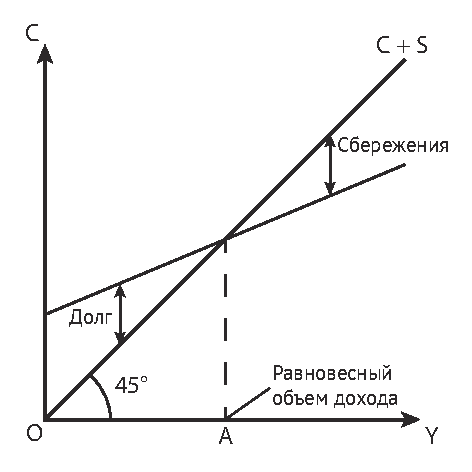
\includegraphics[width=.55\textwidth]{COY}
\end{figure}

В той части, где потребление превышает доход, идет жизнь в долг. Если доход
превышает уровень потребления, то разница образует величину сбережения.

\begin{figure}[h!]
    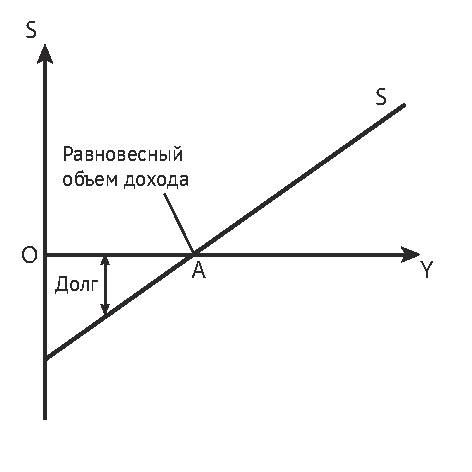
\includegraphics[width=.55\textwidth]{SOY}
\end{figure}

На рисунке изображена кривая сбережений, каждая точка которой равна
вертикальной разнице между биссектрисой и кривой потребления.
 
Мультипликатор оказывает двустороннее действие. Рост инвестиций способствует
мультиплицированному увеличению национального дохода. С другой стороны, даже
небольшое сокращение инвестиций дает резкое и многократное снижение
национального дохода.

Эта закономерность наглядно прослеживается сегодня в российской экономике, где
показатели сокращения объемов капиталовложений в несколько раз меньше
показателей снижения объемов производства и национального дохода.

\begin{figure}[h!]
    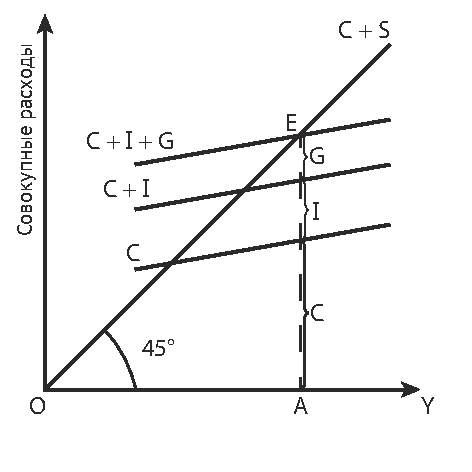
\includegraphics[width=.55\textwidth]{OY}
\end{figure}
 
При наличии государственных расходов равновесный уровень национального дохода
будет соответствовать точке пересечения кривой совокупных расходов
(\( C + I + G \)) и линии \( 45^\circ \), равной сумме потребления и сбережения.

\pagebreak % -------------------------------------------------------------------

\chapter{Особенности действия мультипликатора-акселератора в России}

Согласно теории мультипликатора, рост инвестиций оказывает умноженное
воздействие на доход. Доход возрастает в соответствии с величиной
мультипликатора.

Рост доходов приводит в свою очередь к росту темпов спроса на потребительские
товары и росту их производства. Это вызывает необходимость строительства новых
предприятии по производству потребительских товаров, которое приводит к росту
производства средств производства. Причем рост инвестиций, связанный с
расширением производства средств производства, находится в акселеративной
зависимости от роста доходов, иначе говоря, рост инвестиций равен произведению
коэффициента акселерации на прирост дохода. Это, в свою очередь, приводит в
действие заново весь процесс мультипликации.

Сторонники теории мультипликатора считают, что поскольку рост инвестиций, так
же как и рост спроса на потребительские товары, зависит от государственных
ассигнований, то, следовательно, в руках государства находится решение проблемы
бескризисного развития экономики.

Первоначальные инвестиции, вызывающие эффект мультипликации, носят характер
автономных инвестиций. В отличие от этого принцип акселерации имеет дело со
стимулированными инвестициями, которые зависят от дохода, т.е. являются
результатом возрастания конечного спроса или объема продаж. Автономные
инвестиции дают первоначальный толчок процессу расширения экономики и вызывают
эффект мультипликации, а стимулированные инвестиции, являясь результатом
возросшего дохода, приводят к дальнейшему росту дохода.

Немаловажное значение в механизме действия мультипликатора в России имеет
<<разумная>> правительственная кредитно-денежная и налоговая политика. Банки в
результате перелива капитала из прибыльных в менее прибыльные отрасли, будут
способствовать оживлению предпринимательской деятельности. Затем будут
развиваться третьи, четвертые отрасли. По существу, возникнет <<цепная
реакция>> между отраслями, что и обеспечит рассмотренный эффект
мультипликатора-акселератора.

\pagebreak % -------------------------------------------------------------------

\chapter*{Заключение}
\addcontentsline{toc}{chapter}{Заключение}

В экономической теории многими видными учеными-экономистами рассматривались
проблемы кризисов в предпринимательской деятельности. Российская экономика в
последние годы переживает спад производства в связи с переходом на рыночные
отношения. Отступление от командных методов управления и плановой централизации
хозяйственных операций требует изучения сущности рисков и контроля в управлении
предпринимательской деятельностью в коммерческих банках и фирмах.

Изучая сущности рисков и контроля предпринимательской деятельности можно более
осмысленно разрабатывать экономическую политику государства, а также
прогнозировать экономическую активность на различных фазах цикла. Среди прочего
это способствует повышению эффективности инвестирования, снижению потерь
факторов производства и повышению производительности их использования.

\newpage % ---------------------------------------------------------------------
\renewcommand{\bibname}{Список литературы}

\begin{thebibliography}{99} \addcontentsline{toc}{chapter}{Список литературы}
    \bibitem{1} Экономическая теория: учебник / под общ. ред. В.~И.~Видяпина.
    -- М.: ИНФРА-М, 2007.
    \bibitem{2} Яллай В. А. Макроэкономика. Учеб. Пособие. -- П.: ПГПИ, 2006.
    \bibitem{3} Теплова Т. В. Финансовый менеджмент: управление капиталом и
    инвестициями: учебник для вузов / Т. В. Теплова. М. : ГУ-ВШЭ, 2000.
    \bibitem{4} В. А. Черкасова, О. С. Яковлева. Оценка инвестиций в крупные
    проекты // Корпоративные финансы. 2008.
    \bibitem{5} Инвестиционная деятельность: Учебное пособие / под ред.
    Г.~П.~Подшиваленко и М.~В.~Киселевой. -- М.: ЮНИТИ, 2005. 
    \bibitem{6} Барр Р. Политическая экономия. В 2 т. -- М.: Международные
    отношения, 1994. -- Т. 2, тема II, гл. 2.
    \bibitem{7} История экономических учений: Учебное пособие / Под ред.
    А.~Г.~Худокормова. -- М.: Изд-во МГУ, 1994. -- Ч. II, гл. 10.
    \bibitem{8} Кейнс Дж. М. Общая теория занятости, процента и денег
    // Избранные произведения. -- М.: Экономика, 1993.
    \bibitem{9} Макконнелл К. Р., Брю С. Л. Экономикс: Принципы, проблемы и
    политика. -- М.: Республика, 1992. -- Гл. 13.
    \bibitem{10} Самуэльсон П. Экономика. В 2 т. -- М.: Алгон. 1992. -- Т. 1,
    гл. 13. 
    \bibitem{11} Фишер С., Дорнбуш Р., Шмалензи Р. Экономика. -- М.: Дело Лтд,
    1993. -- Гл. 25.
\end{thebibliography}